\pagenumbering{arabic}
\documentclass[slides]{beamer}
%\documentclass[slides,hyperref={pdfpagelabels=false}]{beamer}
%\documentclass[handout,gray]{beamer}
\usepackage[T1]{fontenc}
\usepackage[utf8]{inputenc}
\usepackage{textcomp}
\usepackage{verbatim}
\usepackage{amsbsy}
\usepackage{multicol}
\usepackage{booktabs} % Make some nice tables
\usepackage{ae,aecompl}


%%%%%%%%%%%%% Simen packages
\usepackage{graphicx, psfig, epsfig}
\usepackage[dvips]{pstcol} % To use the standard "color" package with Seminar
%%%%%\usepackage{semcolor}
 \usepackage{latexsym}
 \usepackage{color}
 \usepackage{amsmath}
 \usepackage{amssymb}
%%%%%%%%%%%%% end Simen packages

%%%%%%%%%%%% COULEURS %%%%%%%%%%%%%%%%%%%%%%%%%%%

\mode<presentation>
{
  \definecolor{beamerstructure}{RGB}{43,79,112}
  \definecolor{sidebackground}{RGB}{230,242,250}
  \definecolor{CTCC}{RGB}{133,188,228}
  \color{beamerstructure}
  \usetheme{default}
  \usepackage{times}
  \beamertemplateballitem
\setbeamertemplate{navigation symbols}{}
%\setbeamertemplate{sidebar left}{\thispdfpagelabel{\insertframenumber}}
%\setbeamertemplate{footline}{\quad\insertframenumber}
%\usecolortheme{CTCC}
}
\usebackgroundtemplate{
\includegraphics[width=1.02\paperwidth]{ctcc_general.jpg}}

\title{\\\vspace{1cm}
Pair-Atomic Resolution-of-the-Identity}
%\subtitle{\textcolor{magenta}{My subtitle (if applicable)}}
\author{Patrick Merlot, Simen Reine and Trygve Helgaker}
%\institute[CTCC]{\\[-6mm]<my.name>@somewhere.no\\[6mm]University of Oslo\\[6mm]
\institute[CTCC]{\\[-6mm]patrick.merlot@kjemi.uio.no\\[6mm]NKS meeting in Computational Chemistry\\[6mm]

\includegraphics[height=1.5cm]{uio.pdf}\hspace{1cm} 

\includegraphics[height=1.5cm]{sff.pdf}\hspace{1cm}

\includegraphics[height=1.5cm]{uit.pdf}}
\date{Trondheim, Norway\\23 nov.2010}

\newcommand{\gb}[1]{green!#1!black}
\newcommand{\rb}[1]{red!#1!black}
\newcommand{\bb}[1]{blue!#1!black}
\newcommand{\coleq}{red!60!black}
\newcommand{\du}{\textrm{d}}

%%%%%%%%%%%%%%%%%%%%%%%
%%%% commands Simen
\definecolor{light}{gray}{0.85}
\DeclareMathOperator{\Tr}{Tr}
\DeclareMathOperator{\erf}{erf}
\DeclareMathOperator{\vek}{vec}
\newcommand{\clr}{\color{red}}
\newcommand{\clg}{\color{green}}
\newcommand{\clb}{\color{blue}}
\newcommand{\clbrown}{\color{brown}}
\newcommand{\slc}{\color{black}}
\newcommand{\eqc}{\color{blue}}
\newcommand{\itc}{\color{blue}}
\newcommand{\emc}[1]{\color{red}#1}
\newcommand{\head}[1]{\begin{center} \fbox{\color{red}#1} \end{center}}
\newcommand{\itm}{\item[\emc $\bullet$]}
\newcommand{\back}{\vspace*{-10pt}}
\newcommand{\mbold}[1]{\ensuremath{\mbox{\boldmath $#1$}}}
\newcommand{\beq}{\begin{equation*}\color{blue}}
\newcommand{\eeq}{\end{equation*}\color{black}}
%
\newcommand{\SlideColours}[2][black]{%
% #1 = foreground color (optional, default=black), #2 = background color
\slideframe[\psset{fillcolor=#2,fillstyle=solid}]{scplain}
\color{#1}}
%
\def\bm#1{\mbox{\boldmath $ #1 $}}
\newenvironment{eec}{\begin{displaymath}\begin{color}{blue}}{\end{color}\end{displaymath}}
%%%%%%%%%%%%%%%%%%%%%%%









\begin{document}
\setlength{\unitlength}{\textwidth}

{
\usebackgroundtemplate{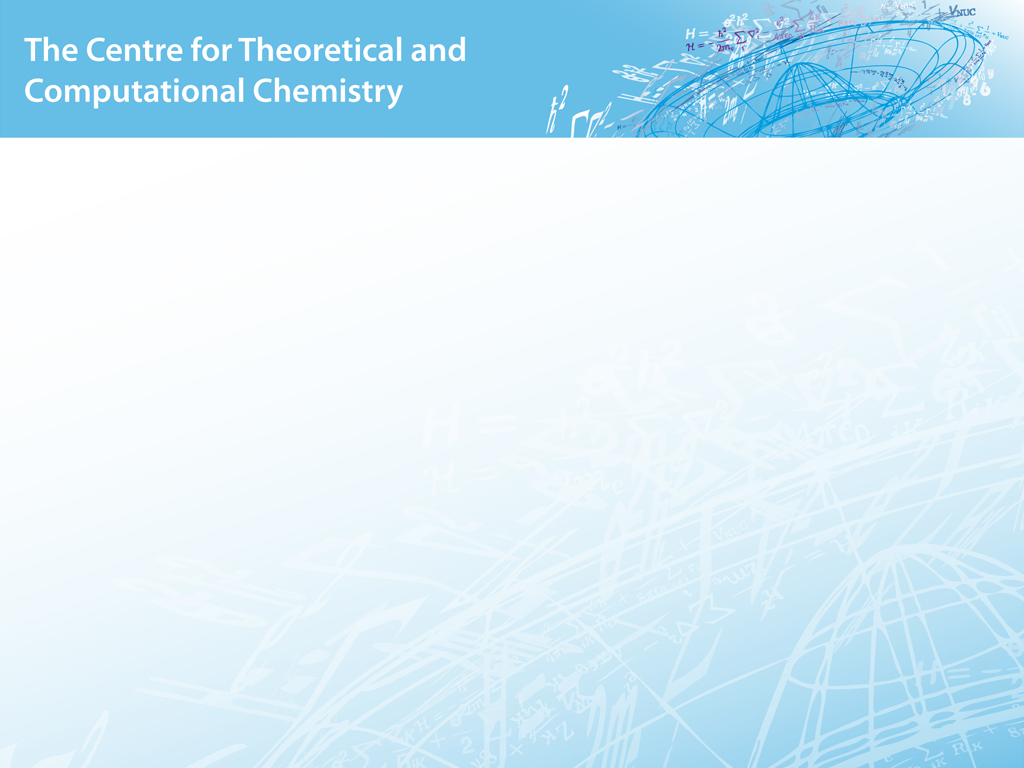
\includegraphics[width=1.02\paperwidth]{ctcc_forside.jpg}}
\maketitle
}

%%%%%%%%%%%%%%%%%%%%%%%%%%%%%%%%%%%%%%%%%%%%%%%%%%%%%%%%%%%%%%%%%%%%%%%%%%%%%%%%%%%%%%%%%%%%%%%%%%%%%
% \begin{frame}{Outline1}
% \begin{itemize}
%  \item \ldots
% \end{itemize}
% \end{frame}


 
\begin{frame}{Outline}
\footnotesize

\begin{itemize}
\item The resolution-of-the-identity approximation
\item Local fitting methods
\item The PARI approximation
\item Preliminary results
\item Conclusion and future perspective
\end{itemize}
\end{frame}
%%%%%%%%%%%%%%%%%%%%%%%%%%%%%%%%%%%%%%%%%%%%%%%%%%%%%%%%%%%%%%%%%%%%%%%%%%%%%%%%%%%%%%%%%%%%%%%%%%%%%
 
\begin{frame}{The RI approximation}
\footnotesize

\begin{itemize}
\item The resolution-of-the-identity (RI), or the {\blue density-fitting} approximation:%, is today commonly use in quantum chemistry
\begin{itemize}
  \item {\blue Speed up calculations (typically by factor 3-30) at little loss of chemical accuracy}
  \item {\blue Highly successful for approximating the Coulomb contribution (in particular in DFT)}
  \item Also used for small- to medium-sized systems for approximation of the exact exchange and 
        in correlated treatment - {\red scaling wall}
  \item {\red Requires an auxiliary basis set}
\end{itemize}
\item In the most commonly used RI treatments, the
     four-center two-electron integrals ${\blue (\mu\nu|\gamma\delta)}$ are 
     approximated by ${\blue \widetilde{(\mu\nu|\gamma\delta)}}$, according to
%
\beq
  (\mu\nu|\gamma\delta) \approx \widetilde{(\mu\nu|\gamma\delta)} 
   = \sum_{IJ} (\mu\nu|I)(I|J)^{-1}(J|\gamma\delta)
\eeq
%
with ${\blue \left\{ \mu \right\}}$ the (regular) AO basis set and with
an atom-centered auxiliary basis set ${\blue \left\{ I \right\}}$ 
%\begin{itemize}
%  \item The Coulomb contribution ({\blue up to 10 000 basis functions})
  \item The Coulomb contribution ({\blue up to 10 000 basis functions})
\beq
\begin{split}
  &J_{\mu\nu} = (\mu\nu|\rho) = \sum_{\gamma\delta} (\mu\nu|\gamma\delta) D_{\gamma\delta}\\
  \approx &\tilde J_{\mu\nu} = (\mu\nu|\tilde\rho) = \sum_{I} (\mu\nu|I)c_I, 
   \quad \red \sum_J (I|J)c_J = (J|\rho)
\end{split}
\eeq
%\end{itemize}

\end{itemize}
\end{frame}

%%%%%%%%%%%%%%%%%%%%%%%%%%%%%%%%%%%%%%%%%%%%%%%%%%%%%%%%%%%%%%%%%%%%%%%%%%%%%%%%%%%%%%%%%%%%%%%%%%%%%
 
\begin{frame}{\small RI for exchange}
\footnotesize
\begin{itemize}
\item The exchange contribution
\begin{eec}
  K_{\mu\nu} = \sum_{\gamma\delta} (\mu\gamma|\nu\delta) D_{\gamma\delta} = \sum_i^\text{occ} (\mu i | \nu i)
\end{eec}
approximated according to - {\blue Wigend (2002), Polly~\emph{et.al} (2004)}
\begin{eec}
  \tilde K_{\mu\nu} = \sum_{\gamma\delta} \sum_{IJ} (\mu\gamma|I)(I|J)^{-1}(J|\nu\delta) D_{\gamma\delta}
                    = \sum_i^\text{occ} \sum_{IJ} (\mu i |I)(I|J)^{-1}(J| \nu i)
\end{eec}
\item {\red Scaling wall} limits this approach to about 1000 basis-functions

\begin{itemize}
  \item metric matrix $\blue (I|J)$ non-sparse $\red \to {\cal O}(N^3)$ scaling
  \item non-locality of fitting coefficients $\blue c_I^{\mu\nu}$
\begin{eec}
  \blue c_I^{\mu\nu} = \sum_J (I|J)^{-1} (J|\mu\nu)
\end{eec}
  \item transformation steps, e.g. 
\begin{eec}
  \blue (I|\mu i) = \sum_{\nu} (I|\mu\nu) L_{\nu i}, \quad {\red {\cal O}(N^2 N_\text{occ})}
\end{eec}
\end{itemize}
\end{itemize}
\end{frame}

%%%%%%%%%%%%%%%%%%%%%%%%%%%%%%%%%%%%%%%%%%%%%%%%%%%%%%%%%%%%%%%%%%%%%%%%%%%%%%%%%%%%%%%%%%%%%%%%%%%%%
 
\begin{frame}{\small Local fitting methods}
\footnotesize
%
\begin{itemize}
\item Two main approaches for linear scaling RI
\begin{itemize}
  \item Partition density and fit each density in a local region - {\blue Gallant and St-Amant (1996),
        Sodt~\emph{et.al} (2006), Sodt and Head-Gordon (2008)}
%\begin{eec}
%  \rho(\mathbf{r}) = \sum_s \rho^s(\mathbf{r}), \quad \red \rho^s(\mathbf{r}) \approx \tilde\rho^s(\mathbf{r})
%\end{eec}
  \item Obtain fitting coefficients using local metric - {\blue Baerends~\emph{et.al} (1973), Vahtras~\emph{et.al} (1993), Jung~\emph{et.al} (2005), Reine~\emph{et.al} (2008)}
\begin{eec}
  c_I^{\mu\nu} = \sum_J \langle I|w|J \rangle^{-1} \langle J|w|\mu\nu\rangle
\end{eec}
\end{itemize}
\item In the atomic RI (ARI) approaches of Sodt~\emph{et.al} each charge distribution $\blue |\mu\nu)$ is 
     first associated with a center $\blue C$, and is fitted using auxiliary functions 
     $\blue |I)$ centered on the atoms in some buffer zone $\blue [C]$ around $\blue C$ 
     %({\blue Coulomb metric})
\begin{eec}
  |\mu\nu) = \sum_I c_I^{\mu\nu} |I), \quad \red |I) \in [C]
\end{eec}
\begin{itemize}
  \item fixed buffer-zone size - {\red system dependent}
  \item the set $\blue |I)$ includes the auxiliary functions centered on {\red several atoms}
\end{itemize}
\item Jung~\emph{et.al} explored the decay behavior of the two-center fitting coefficients
     $\blue c_I^{\mu\nu}$. 
\begin{itemize}
    \item Coulomb metric fit - the asymptotic decay of $\blue c_I^{\mu\nu}$ was as slow 
          as $\blue \frac{1}{r}$
    \item local ({\blue overlap/attenuated Coulomb}) metric fit - exponential decay with distance
\end{itemize}
\end{itemize}

\end{frame}
%%%%%%%%%%%%%%%%%%%%%%%%%%%%%%%%%%%%%%%%%%%%%%%%%%%%%%%%%%%%%%%%%%%%%%%%%%%%%%%%%%%%%%%%%%%%%%%%%%%%%
 
\begin{frame}{\small The PARI approach}
\footnotesize
\begin{itemize}
\item We propose the pair-atomic resolution-of-the-identity (PARI)
\begin{itemize}
\item fit each charge distribution $\blue |\mu\nu)$ with auxiliary functions
     $\blue |I)$ centered on the two parent atoms $\blue A$ and $\blue B$ of 
     the basis functions $\blue |\mu)$ and $\blue |\nu)$
\begin{eec}
  |\widetilde{\mu\nu}) = \sum_{I\in{A\cup B}} c_I^{\mu\nu}|I), 
   \quad \red c_I^{\mu\nu} = \sum_{J\in{A\cup B}} (I|J)^{-1}(J|\mu\nu)
\end{eec}
\item replace all $\blue (\mu\nu|\gamma\delta)$ by {\red robust} and {\red variational} 
      $\blue \widetilde{(\mu\nu|\gamma\delta)}$ given by
\begin{equation*}
\begin{split}
\blue
  \widetilde{(\mu\nu|\gamma\delta)} &\blue= (\mu\nu|\widetilde{\gamma\delta}) 
    + (\widetilde{\mu\nu}|\gamma\delta) - (\widetilde{\mu\nu}|\widetilde{\gamma\delta})\\
& = \blue (\mu\nu|\gamma\delta) - \red (\mu\nu-\widetilde{\mu\nu}|\gamma\delta-\widetilde{\gamma\delta})
\end{split}
\end{equation*}
\item {\blue highly local}
\item {\blue removes scaling bottleneck }
\item {\red decreases accuracy} $\to$ larger auxiliary basis sets
\end{itemize}
\item PARI-J for the Coulomb contribution
\begin{eec}
  \widetilde{J}_{\mu\nu} = \sum_I (\mu\nu|I)c_I + \sum_{I\in{A\cup B}} c_I^{\mu\nu}(I|\rho-\tilde\rho),
\quad \red c_I = \sum_{\gamma\delta} c_I^{\gamma\delta} D_{\gamma\delta}, \quad 
\blue |\tilde\rho) = \sum_I c_I|I)
\end{eec}
\begin{itemize}
  \item straightforwardly linear scaling using screening and FMM
\end{itemize}
\end{itemize}
\end{frame}
%
%%%%%%%%%%%%%%%%%%%%%%%%%%%%%%%%%%%%%%%%%%%%%%%%%%%%%%%%%%%%%%%%%%%%%%%%%%%%%%%%%%%%%%%%%%%%%%%%%%%%
 
\begin{frame}{\small PARI-K}
\footnotesize
\begin{itemize}
\item PARI applied to the exchange term (PARI-K) 
\begin{itemize}
\item split fitting coefficients into the two parent atoms
\begin{eec}
  |\widetilde{\mu\nu}) = 
  |\widetilde{\underbar{$\mu$}\nu}) + |\widetilde{\mu\underbar{$\nu$}}), 
  \quad \red |\widetilde{\underbar{$\mu$}\nu}) = \sum_{I\in A} c_I^{\mu\nu} |I),
  \quad \blue |\mu\widetilde{\underbar{$\nu$}}) = \sum_{J\in B} c_J^{\mu\nu} |J)
\end{eec}
\item leads to a splitting of $\blue \widetilde{(\mu\nu|\gamma\delta)}$ into eight parts
      - four involving three-center and four two-center integrals
\item collect terms in order to calculate each integral only once and select 
      contraction pathway in order to reduce cost
\item exploit symmetry of integrals and density matrix 
\end{itemize}
\item An example three-center term
\begin{equation*}
 \blue K_{\mu\gamma} \stackrel{+}{=} \sum\limits_{I\delta} d_{I,\delta}^\mu (I|\gamma\delta), 
  \quad \red I,\mu\in A,\blue \gamma\in C, \red \delta\in {\cal M}, \quad
  \blue d_{I,\gamma}^\mu = \sum\limits_\nu c_I^{\mu\nu}D_{\nu\gamma}
%\begin{split}
% \blue K_{\mu\gamma} &\blue\stackrel{+}{=} \sum\limits_{I\delta} d_{I,\delta}^\mu (I|\gamma\delta), \quad \red I,\mu\in A,\blue \gamma\in C, \red \delta\in {\cal M}\\
% \blue d_{I,\gamma}^\mu &\blue = \sum\limits_\nu c_I^{\mu\nu}D_{\nu\gamma}
%\end{split}
\end{equation*}
\begin{itemize}
  \item ignoring screening each of these terms scale $\blue {\cal O}(N^3 n^3 a)$ with number of
        the number of atoms $\blue N$ and regular and auxiliary basis functions per atom 
        $\blue n$ and $\blue a$
  \item to be compared with the $\red {\cal O}(N^4 n^2 a^2)$ scaling of conventional RI - {\blue can 
        be reduced to $\red {\cal O}(N^3 N_\text{occ} n a^2)$ using MOs, with $\red N_\text{occ}$ 
        the number of occupied MOs}
\end{itemize}
%\item Note that PARI-K can be modified to include MO-transformations as well
\end{itemize}
\end{frame}
%
%%%%%%%%%%%%%%%%%%%%%%%%%%%%%%%%%%%%%%%%%%%%%%%%%%%%%%%%%%%%%%%%%%%%%%%%%%%%%%%%%%%%%%%%%%%%%%%%%%%%%

\begin{frame}{\small Outline of PARI-K algorithm}
\footnotesize
\begin{figure}
\begin{tabbing}
\hspace{3pt}\=\hspace{10pt}\=\hspace{10pt}\=\hspace{10pt}\=\hspace{10pt}\=\hspace{10pt}\=\hspace{10pt}\=\hspace{10pt}\=\hspace{10pt}\=\hspace{10pt}\kill
\> {\blue Three-center contributions} \\
\> Loop $A$ \\
\> \> Calculate the fitting coefficients $\blue c_I^{\mu\nu}, \quad \red I,\mu\in A, \blue \nu\in {\cal M}$ and density coefficients $\blue d_{I,\gamma}^\mu $ \\
%\> \> Construct density coefficients $\blue d_{I,\gamma}^\mu $\\
\> \> Loop $C$ \\
\> \> \> Loop $D\ge C$ \\
\> \> \> \> Calculate $\blue (I|\gamma\delta), \quad \red I\in A,\blue\gamma\in C, \red\delta\in D$ \\
\> \> \> \> Make contractions \\
\> \> \> \> \> $\blue \tilde K_{\mu\gamma} \stackrel{+}{=} \sum\limits_{I\delta} d_{I,\delta}^\mu (I|\gamma\delta), \red \quad {\cal O}(N^3 n^3 a)$ \\
\> \> \> \> \> $\blue \tilde K_{\mu\delta} \stackrel{+}{=} \sum\limits_{I\gamma} d_{I,\gamma}^\mu (I|\gamma\delta), \red \quad {\cal O}(N^3 n^3 a)$ \\
\> \> \> \> \> $\blue X_{I,\gamma}^\mu = \sum\limits_\delta (I|\gamma\delta)D_{\mu\delta}, \red \quad {\cal O}(N^3 n^3 a)$ \\
\> \> \> \> \> $\blue X_{I,\delta}^\mu = \sum\limits_\gamma (I|\gamma\delta)D_{\mu\gamma}, \red \quad {\cal O}(N^3 n^3 a)$ \\
%\> \> \> End loop $D$ \\
\> \> Make contractions \\
\> \> \> $\blue \tilde K_{\nu \gamma} \stackrel{+}{=} \sum_{I,\mu} c_{I}^{\mu\nu} X_{I,\gamma}^\mu, \red \quad {\cal O}(N^3 n^3 a)$ \\
\> \> \> $\blue \tilde K_{\nu \delta} \stackrel{+}{=} \sum_{I,\mu} c_{I}^{\mu\nu} X_{I,\delta}^\mu, \red \quad {\cal O}(N^3 n^3 a)$ \\
%\> \> End loop $C$ \\
%\> End loop $A$ \\
\> Symmetrized or anti-symmetrized $\blue \mathbf{\tilde K}$ \\
\end{tabbing}
\end{figure}
\end{frame}


 
\begin{frame}{\small Example results}
\footnotesize
\begin{center}
Naphtalene, B3LYP, cc-pVTZ/cc-pVTZdenfit 
\begin{tabular}{lcccc}
\hline 
           & Energy    &  Error        & Time/iter  \\ 
           & (Hartree) &  (micoHartree) & (s)       \\ 
\hline
{Regular}  &   -385.775114        &  0 &  1998  \\
{RI}       &   -385.7751{\red 66} & 52 &   {\blue 362}  \\
{PARI}     &   -385.775{\red 203} & 89 &   736  \\
\hline
\end{tabular}
\end{center}
\end{frame}


\begin{frame}{\small Conclusion and future perspective}
\footnotesize
\begin{itemize}
\item We have presented the PARI scheme for efficient calculation of the Coulomb 
     and exchange contributions to DFT
\item The PARI method can in general be used for any method involving four-center two-electron
     integrals
\item Linear scaling in nature
\item Allows differentiated treatment by adding Lagrangian multipliers
\item Some work remains to fully test both accuracy and efficiency
\item Preliminary results are highly promising
\end{itemize}
\begin{center}
{\red Thank you for your attention!}
\end{center}
\end{frame}
%
%%%%%%%%%%%%%%%%%%%%%%%%%%%%%%%%%%%%%%%%%%%%%%%%%%%%%%%%%%%%%%%%%%%%%%%%%%%%%%%%%%%%%%%%%%%%%%%%%%%%%




% \begin{frame}{Outline1}
% \begin{itemize}
%  \item \ldots
% \end{itemize}
% \end{frame}

% \begin{frame}{Outline2}
% \begin{itemize}
%  \item \ldots
% \end{itemize}
% \end{frame}

% \begin{frame}{Outline3}
% \begin{itemize}
%  \item \ldots
% \end{itemize}
% \end{frame}

\end{document}